\chapter{深度学习}
\label{chap:deeplearning}

由神经元提出的感知机模型,只适用于解决二分类问题,对于多分类却无能为力,
而多层感知机却能解决这个问题。

\begin{figure}[!htb]
	\centerline{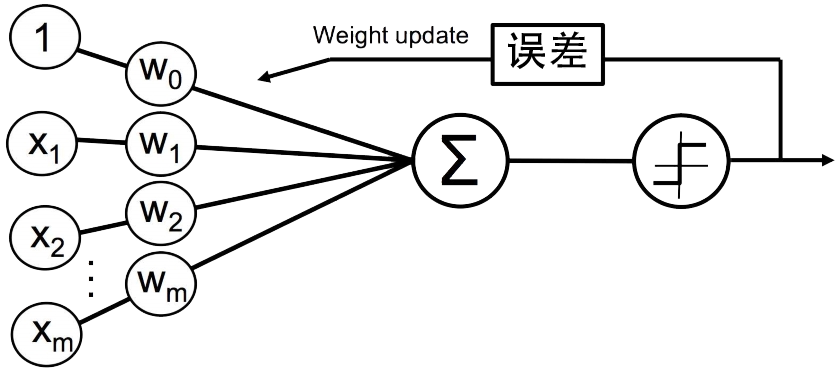
\includegraphics[width=.25\figwidth]{images/perceptron.png}}
	\label{fig:part2_perceptron}
	\caption{感知机}
\end{figure}

\noindent
我们知道感知机可以实现AND、OR、NAND逻辑,而XOR正好可以由它们推算得出:
$x1\;\oplus\;x2 = (x1\;|\;x2)\;\&\;(x1\;\bar{\&}\;x2)$

\begin{figure}[!htb]
	\centerline{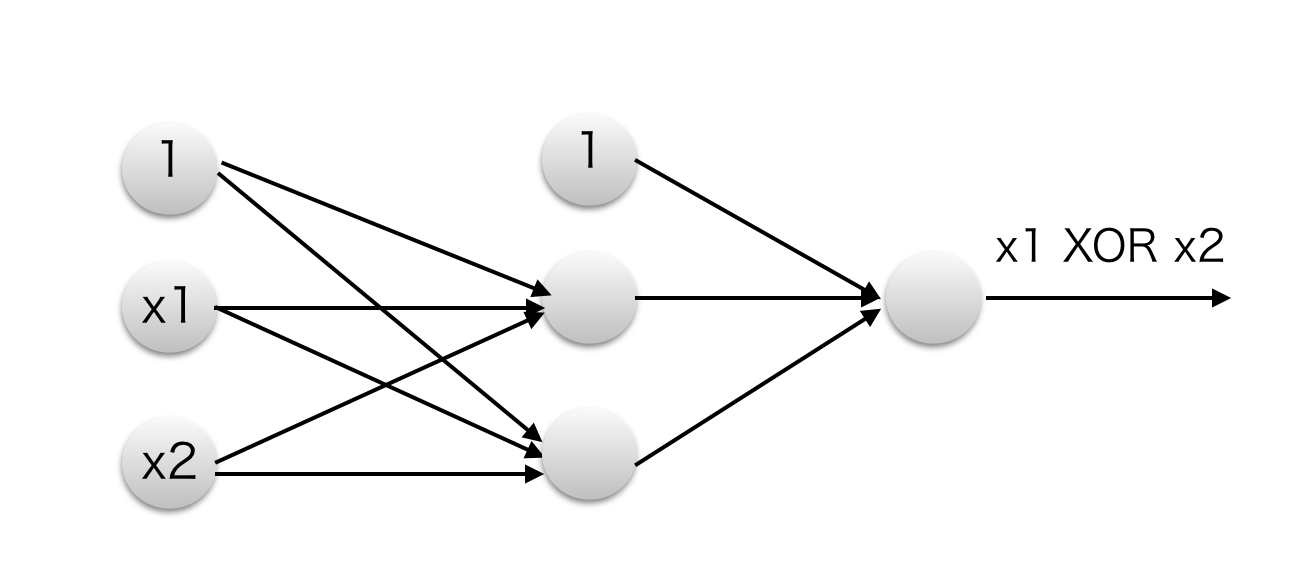
\includegraphics[width=.25\figwidth]{images/xor.png}}
	\label{fig:part2_xor}
	\caption{异或}
\end{figure}

\noindent
这就是深度学习的魅力,但为什么在感知机提出来之后却停滞发展二十年呢?
对于普通的二分类问题,使用的损失函数是基于点线距离的,但毕竟不是一个通用的解决方案。
用于解决多分类问题的时候,就会显得非常笨重,越来越不好用。
实际上,感知机和SVM非常相似,主要差别在于超平面(分割线)是否唯一,是否满足间隔最大化。
感知机是不要求间隔最大的,只要能分开数据就算解决了。

\section{多层感知机}
本节以XOR为例,作为深度学习的入门铺垫。
已知,单层感知机是可以实现AND、OR、NAND逻辑功能的。
如下图:


\begin{figure}[!htb] \centering 
	\begin{tikzpicture}
		\node at (0,0) {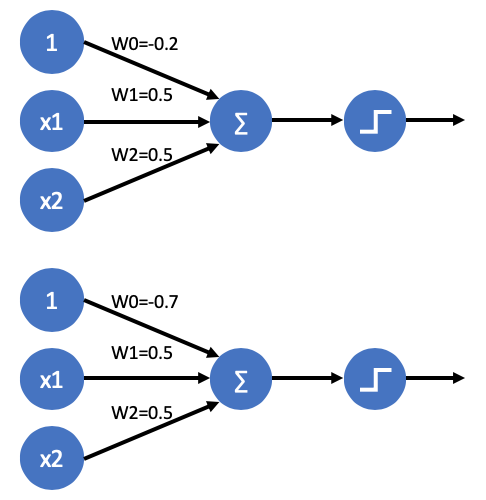
\includegraphics[width=6cm]{images/perceptron_and_or.png}};
		\node at (4,1.6) {逻辑OR};
		\node at (5.5,1) {\small{\(1,0\)=>真,\(1,1\)=>真,\(0,0\)=>假}};
		\node at (4,-1.6) {逻辑AND};
		\node at (5.5,-2.2) {\small{\(1,0\)=>假,\(1,1\)=>真,\(0,0\)=>假}};
	\end{tikzpicture}
	\caption{感知机模型:AND、OR}
\end{figure}

\noindent
感知机的参数如上,我们定义了AND和OR的运算模型,而NAND是AND相反运算,
只要把上图AND的参数都取反即可:$(0.5, 0.5, 0.7) \Rightarrow (-0.5, -0.5, 0.7)$。
示意图,如下。
\begin{figure}[!htb]
	\centerline{
\includegraphics[width=.25\figwidth]{images/xor_or_nand.png}}
	\label{fig:part2_xor_or_nand}
	\caption{多层感知机求解异或}
\end{figure}

\noindent
感知机的最大缺点是误差计算是基于经验的(点到直线距离),而不是基于输出结果。
如果误差的调节,能反应到$w$和$b$,势必要求整个调整过程是可微的,也就是一个平滑的过程。
这个平滑的调节就是基于偏导数实现的,也就是梯度。
因此,这也要求从输入到输出,从误差到输入是一个可以微调的平滑过程,这样才有利于机器学习。
实际上,这就是一个迭代求极值点的过程,直到误差最小或者迭代次数到达。
所谓的前向传播和反向传播,就是这个道理。


\begin{figure}[!htbp]
	\centering
	\begin{minipage}{0.33\textwidth}
	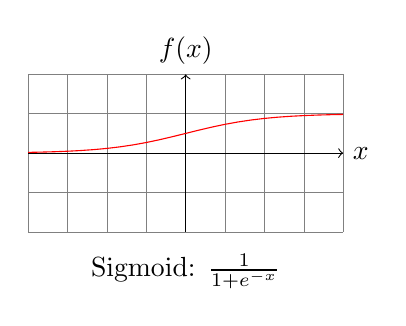
\begin{tikzpicture}[scale=0.5]
		\draw[very thin,color=gray] (-4,-2) grid (4,2);
		\draw[->] (-4,0) -- (4,0) node[right] {$x$};
		\draw[->] (0,-2) -- (0,2) node[above] {$f(x)$};
		\draw[color=red, domain=-4:4] plot (\x,{1/(1+e^-\x)});
		\node at (0, -3) {Sigmoid: $\frac{1}{1+e^{-x}}$};
	\end{tikzpicture}
	\end{minipage}%
	\begin{minipage}{0.33\textwidth}
	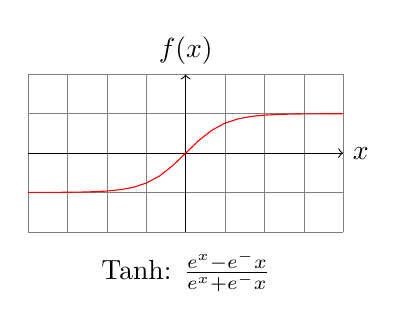
\begin{tikzpicture}[scale=0.5]
		\draw[very thin,color=gray] (-4,-2) grid (4,2);
		\draw[->] (-4,0) -- (4,0) node[right] {$x$};
		\draw[->] (0,-2) -- (0,2) node[above] {$f(x)$};
		\draw[color=red, domain=-4:4] plot (\x,{(e^\x-e^-\x)/(e^\x+e^-\x)});
		\node at (0, -3) {Tanh: $\frac{e^x-e^-x}{e^x+e^-x}$};
	\end{tikzpicture}
	\end{minipage}%
	\begin{minipage}{0.33\textwidth}
		\vspace{0.55cm}
		\begin{tikzpicture}[scale=0.5]
			\draw[very thin,color=gray] (-4,-2) grid (4,2);
			\draw[->] (-4,0) -- (4,0) node[right] {$x$};
			\draw[->] (0,-2) -- (0,2) node[above] {$f(x)$};
			\draw[color=red, domain=-4:0] plot (\x,0);
			\draw[color=red, domain=0:2] plot (\x,\x);
		\node at (0, -3.2) {ReLu: 
				$\begin{cases} 
					x&\text{x>=0}\\0&\text{x<0}
				\end{cases}$};
		\end{tikzpicture}
	\end{minipage}%
\end{figure}

感知机的缺点来源于激活函数是阶跃函数$Sign$,它不是连续可导的函数,无法微调误差。
换成$ReLu, Simoid, TanH$就可以让感知机重获新生。
输出结果不再是$0$和$1$而是$(0,1)$之间的概率值,代表更应该是哪个结果。

\section{PlayGround}
PlayGround是一个在线演示神经网络的平台,是一个入门神经网络非常直观的网站。
它图形化地展示神经网络的训练过程,非常有利于初学者获得感性认识。
PlayGround演示页面由
DATA(数据)、FEATURES(特征)、HIDDEN LAYERS(隐含层)、OUTPUT(输出层),
四个部分组成。

在DATA一栏里提供了4种不同形态的数据,分别是圆形、异或、高斯和螺旋。
还可以对这些数据进行配置:噪声、训测比、批大小(Batch)。
平面内的数据分为蓝色和黄色两种。